\documentclass{standalone}
\usepackage{tikz}
\usetikzlibrary{shapes.geometric, arrows.meta, positioning, fit}

\begin{document}
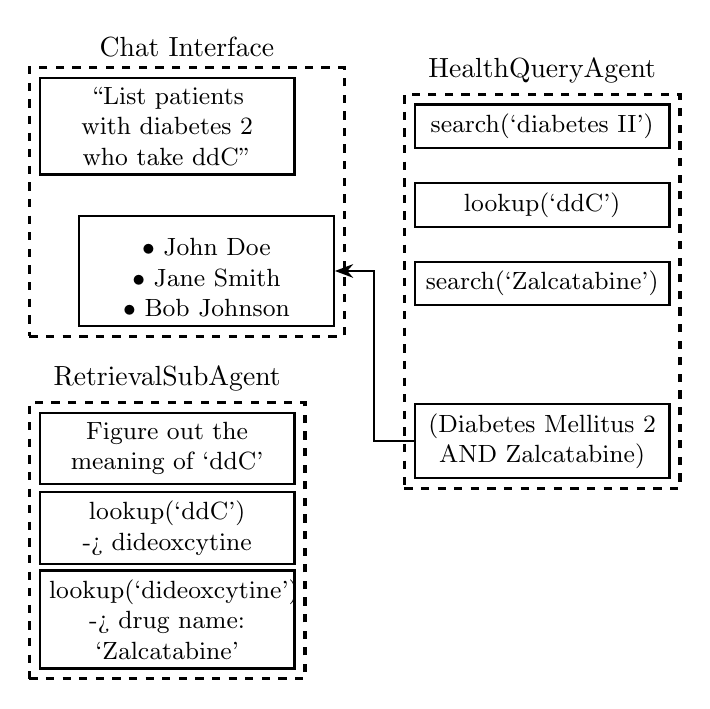
\begin{tikzpicture}[
    node distance=1.5cm,
    innerbox/.style={rectangle, draw, thick, minimum width=2.8cm, minimum height=0.5cm, align=center, text width=3cm, font=\small},
    outerbox/.style={rectangle, draw, very thick, dashed, minimum width=3.5cm, minimum height=2cm},
    databox/.style={rectangle, draw, thick, minimum width=1cm, minimum height=0.6cm, align=center, text width=1.2cm, font=\tiny},
    arrow/.style={-Stealth, thick}
]

% User Interface components
\node[innerbox] (request) {``List patients with diabetes 2 who take ddC''};
\node[innerbox, below=0.5cm of request, xshift=+0.5cm] (response) {\\$\bullet$ John Doe\\$\bullet$ Jane Smith\\$\bullet$ Bob Johnson};

% Processing components

\node[innerbox, right=1.5cm of request, yshift=-0cm] (search1) {search(`diabetes II')};
\node[innerbox, right=1.5cm of request, yshift=-1cm] (lookup) {lookup(`ddC')};
\node[innerbox, right=1.5cm of request, yshift=-2cm] (search2) {search(`Zalcatabine')};

\node[innerbox, right=1.5cm of request, yshift=-4cm] (backend) {(Diabetes Mellitus 2 AND Zalcatabine)};

% Retrieval Sub-agent
\node[innerbox, below=3cm of request] (retrieval1) {Figure out the meaning of `ddC'};
\node[innerbox, below=4cm of request] (retrieval2) {lookup(`ddC') -> dideoxcytine};
\node[innerbox, below=5cm of request] (retrieval3) {lookup(`dideoxcytine') -> drug name: `Zalcatabine'};
% Data layer components

%\node[databox, right=0.5cm of backend, yshift=-0cm] (warehouse) {Data\\Warehouse};
%\node[databox, right=0.5cm of backend, yshift=-2cm] (knowledge) {Knowledge\\Base};
%\node[outerbox, fit=(warehouse) (knowledge), label=above:Data Layer] (datalayer) {};


% Grouping boxes
\node[outerbox, fit=(request) (response), label=above:Chat Interface] (interface) {};
\node[outerbox, fit=(search1) (search2) (lookup) (backend), label=above:HealthQueryAgent] (processing) {};
\node[outerbox, fit=(retrieval1) (retrieval2) (retrieval3), label=above:RetrievalSubAgent] (retrieval) {};
% Clockwise arrows
\draw[arrow] (backend.west) -| ([xshift=0.5cm]response.east) -- (response.east);

\end{tikzpicture}
\end{document}
